\begin{frame}
\frametitle{Principle of spin-coherence time measurement}
\framesubtitle{}

\begin{figure}
              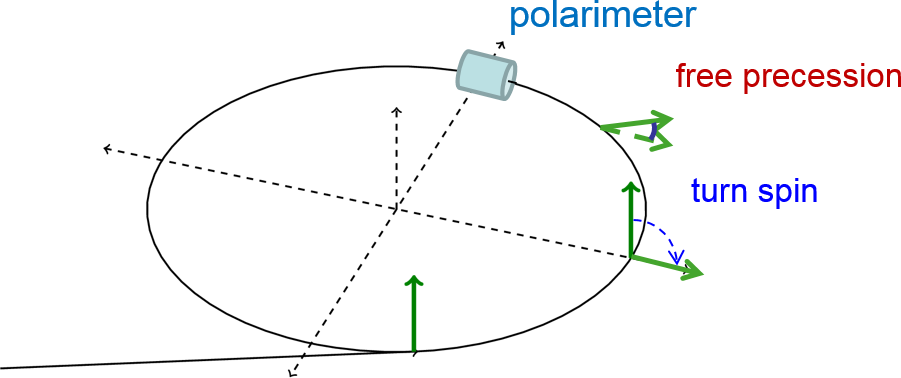
\includegraphics[height=0.27\textheight]{SCT-setup.png}
              \hspace{0.4cm}
			 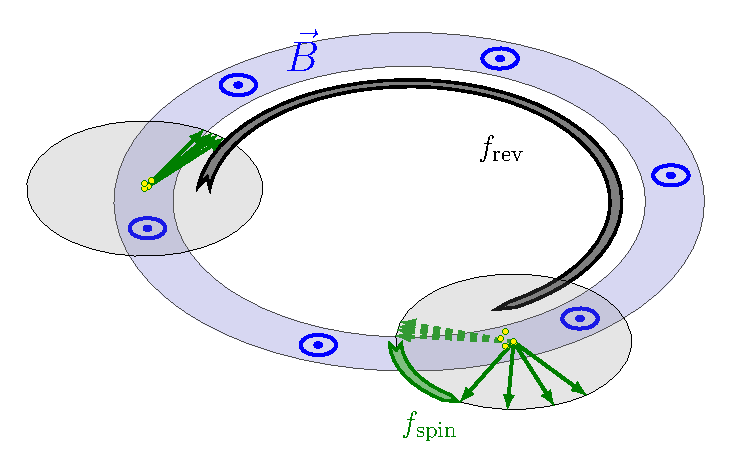
\includegraphics[height=0.29\textheight]{spintune.pdf}
\end{figure}

\begin{block}{Measurement procedure:}
\begin{enumerate}
 \item Vertically polarized deuterons stored at $p \simeq \SI{1}{GeV.c^{-1}}$.
 \item Polarization flipped into horizontal plane with RF solenoid ($\approx \SI{200}{ms}$). 
 \item Beam extracted on Carbon target with ramped bump or by heating.
 \item Horizontal (in-plane) polarization determined from $U-D$ asymmetry.
\end{enumerate}
\end{block}

\end{frame}